\subsection{Tracking downloads with different speeds}
In this experiment we measure if MultiChain can correctly track the upload and download amounts
between two peers with different speeds.
In the scenario a file of 100 MB is downloaded at different speeds,
respectively 500 KB/s, 750 KB/s, 1000 KB/s, 1250 KB/s, 2000 KB/s, and 3000 KB/s.
The maximum speed of anonymous download was measured in experiments to be 1150 KB/s\cite{ruigrok-anonymous}.
The scheduler waits for 1MB uploaded to another peer before scheduling a block.
The upload and download of the file is done by different pairs of seeders and leechers.
Every second these amounts are indicated to have been transferred to the schedulers of every peer.

\begin{figure}
\centering
\subfigure[Total download amount.]{
\centerline{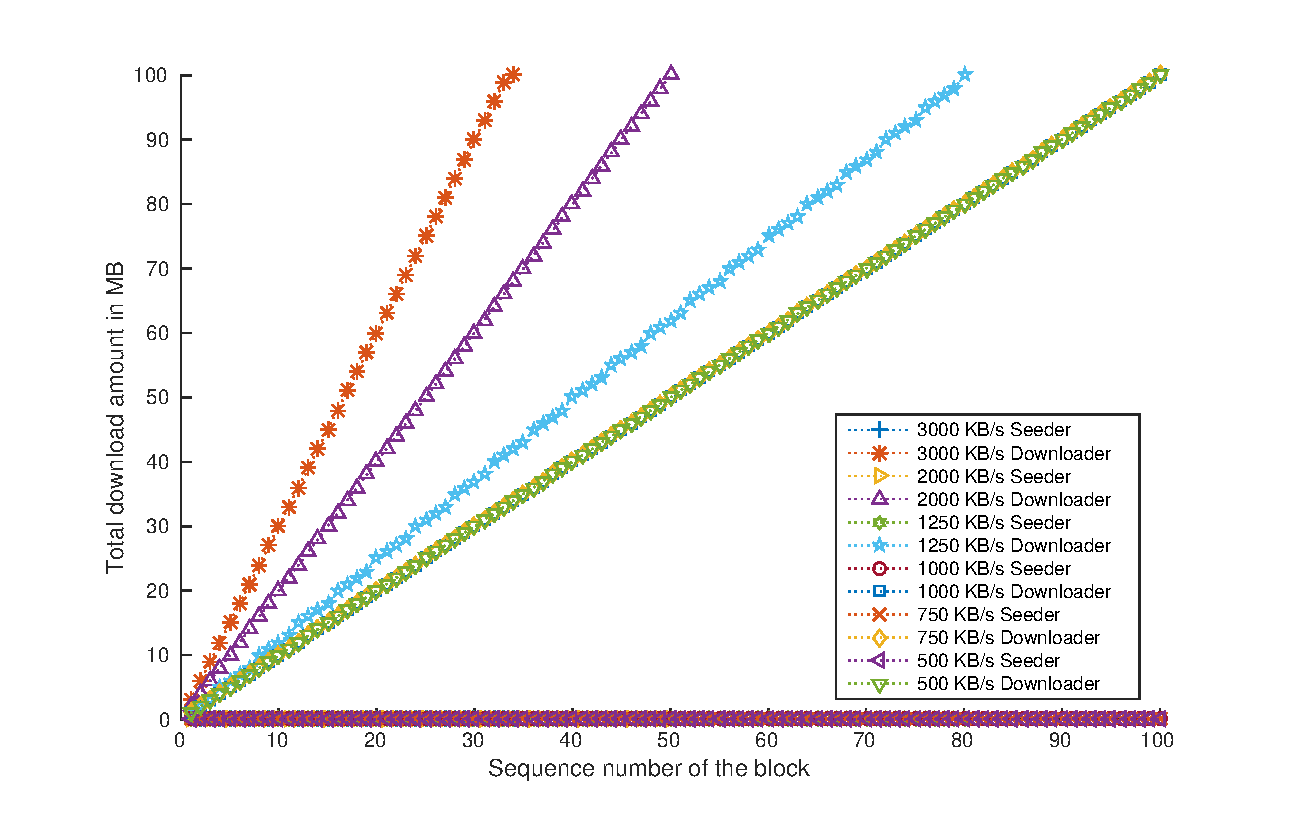
\includegraphics[scale=0.5]{experimentation/speeds/synthetic-simple-down.eps}}
\label{fig:synthetic-simple-down}
}
\subfigure[Total upload amount.]{
\centerline{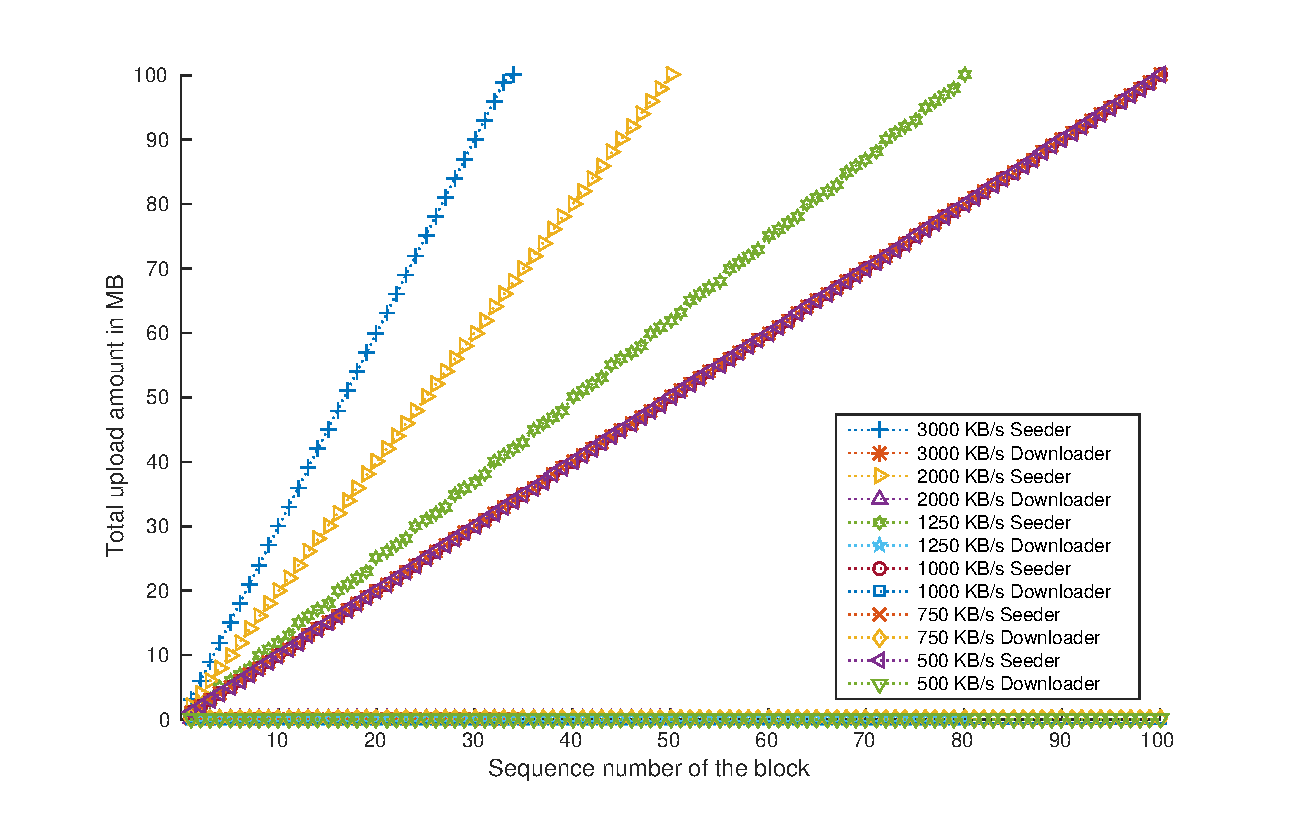
\includegraphics[scale=0.5]{experimentation/speeds/synthetic-simple-up.eps}}
\label{fig:synthetic-simple-up}
}
\caption{Download and upload amounts when tracking downloads at different speeds.}
\label{fig:synthetic-simple-amounts}
\end{figure}

The total download and upload amounts of every peer is plotted in Figure \ref{fig:synthetic-simple-amounts}.
These amounts are plotted in the same way as the previous experiment.
The plots show that MultiChain is able to correctly track the download and upload amounts without a problem.
There are no hitches in the figures and the amounts go up in fixed increments corresponding to the different speeds.
This means that MultiChain is fast enough to correctly track the amounts.

The download speeds below the threshold of 1000 MB of the scheduler
are not distinguishable from the download at the threshold speed.
This is because the scheduler waits until the threshold is reached before initiating the block.
The amount is tracked in the same amount of blocks,
but the total time of the experiment is longer for these experiments.
If the speed goes above the threshold, then this is reflected in the figure.

The graph in Figure \ref{fig:synthetic-simple-graph} shows the graph of the blocks created by the experiment.
The graph is disconnected, because the different pairs of seeders and leechers did not interact with each other.
So no block that would connect their chains is created,
This leaves the graph disconnected.

\begin{figure}
	\centerline{\includegraphics[scale=0.06]{experimentation/speeds/synthetic.png}}
	\caption{Disconnected chain graph of tracking downloads at different speeds.}
	\label{fig:synthetic-simple-graph}
\end{figure}

This experiment was run several times before the final version in this report was run.
Earlier versions of the experiment resulted in two bugfix and two improvements:
the ability of the scheduler to create a block at the end of a download.